\section{Empirical Evaluation and Results}
\label{sec:results}

We report the experimental evaluation organized by research questions RQ1 through RQ5.

\subsection{RQ1: Feasibility and Parity}
Across all evaluated datasets and payload sizes, the end-to-end pipeline deterministically achieved $100.0\%$ bitwise reconstruction parity:
\begin{equation}
\text{SHA-256}(S_{\text{reconstructed}}) \equiv \text{SHA-256}(S_{\text{canonical}})
\end{equation}
Roundtrip reconstruction succeeded for all evaluated trials with zero byte discrepancies. This is a correctness result, not a statistical significance test. On Ethereum Sepolia, transaction \texttt{0x9631...7ea} successfully committed versioned hash \texttt{0x010e...af11} matching the locally generated sidecar. The smart contract suite validated all state invariants, passing 36 Foundry test suites (including 1,024-run fuzzing and 16,384-call stateful invariant campaigns) and 49 Pytest test cases without failure.

\subsection{RQ2: Economics and Break-Even Blob Fees}
% Auto-generated from summary_local_matrix.csv
\begin{table*}[t]
\centering
\small
\caption{Local Evaluation Matrix Across Scientific and Synthetic Datasets [Measured locally]}
\label{tab:local_matrix}
\begin{tabular}{lrrrrrrr}
\hline
Dataset & Canonical Size & Comp. Size & Ratio & Blobs & Waste & Encoding Latency & Throughput \\
& (KiB) & (KiB) & & Count & (\%) & Mean $\pm$ SD (ms) & (MiB/s) \\
\hline
OpenAlex Scholarly Works Metadata & 266.6 & 51.4 & 5.19$\times$ & 1 & 59.8\% & 1.50 $\pm$ 0.09 & 173.1 \\
Atmospheric \& Environmental Sensor Observations & 1027.3 & 101.6 & 10.11$\times$ & 1 & 20.6\% & 3.00 $\pm$ 0.20 & 334.1 \\
Transformer Model Training Step Trace & 518.9 & 89.8 & 5.78$\times$ & 1 & 29.8\% & 2.63 $\pm$ 0.15 & 192.4 \\
Deterministic Scaling Synthetic Dataset (110 KiB) & 110.5 & 12.5 & 8.85$\times$ & 1 & 90.2\% & 0.55 $\pm$ 0.04 & 197.8 \\
Deterministic Scaling Synthetic Dataset (1137 KiB) & 1137.5 & 129.7 & 8.77$\times$ & 2 & 49.3\% & 4.48 $\pm$ 0.37 & 248.0 \\
Deterministic Scaling Synthetic Dataset (5712 KiB) & 5712.6 & 654.5 & 8.73$\times$ & 6 & 14.8\% & 31.72 $\pm$ 0.67 & 175.9 \\
Deterministic Scaling Synthetic Dataset (22909 KiB) & 22909.4 & 2614.8 & 8.76$\times$ & 22 & 7.2\% & 300.23 $\pm$ 4.20 & 74.5 \\
Incompressible Pseudo-Random Binary Negative Control & 1024.0 & 1024.0 & 1.00$\times$ & 9 & 11.1\% & 15.89 $\pm$ 0.71 & 62.9 \\
\hline
\end{tabular}
\end{table*}


Table~\ref{tab:local_matrix} reports the local evaluation matrix. For uncompressed 1.0~MiB payloads, blobs require 9 blobs costing \$27.24~USD versus \$755.92~USD in calldata---a \textbf{$27.8\times$ theoretical cost reduction}. When compression is applied to structured scientific and synthetic data, the economic advantage expands:
\begin{itemize}
    \item \textbf{OpenAlex Scholarly Metadata} (272.9~KiB canonical): Achieves a $5.19\times$ compression ratio down to 52.6~KiB, fitting entirely within a single blob. Cost is \$1.73~USD in blobs versus \$38.85~USD in calldata (\textbf{$22.4\times$ cost reduction}).
    \item \textbf{Synthetic NOAA Climate Observations} (1,051.9~KiB canonical): Compresses $10.11\times$ to 104.1~KiB, fitting into 1 blob costing \$1.73~USD versus \$75.86~USD in calldata (\textbf{$43.8\times$ cost reduction}).
    \item \textbf{Synthetic PyTorch ML Training Trace} (531.3~KiB canonical): Compresses $5.78\times$ to 92.0~KiB, fitting into 1 blob costing \$1.73~USD versus \$67.16~USD in calldata (\textbf{$38.8\times$ cost reduction}).
\end{itemize}

The analytical break-even blob base fee $B^*$ at a 15~gwei execution base fee is $207.9$~gwei. Under prevailing Ethereum mainnet conditions where the blob base fee frequently remains below 10~gwei, blobs provide consistent orders-of-magnitude savings over calldata.

\subsection{RQ3: Performance, Scalability, and Ablations}
\begin{figure}[t]
\centering
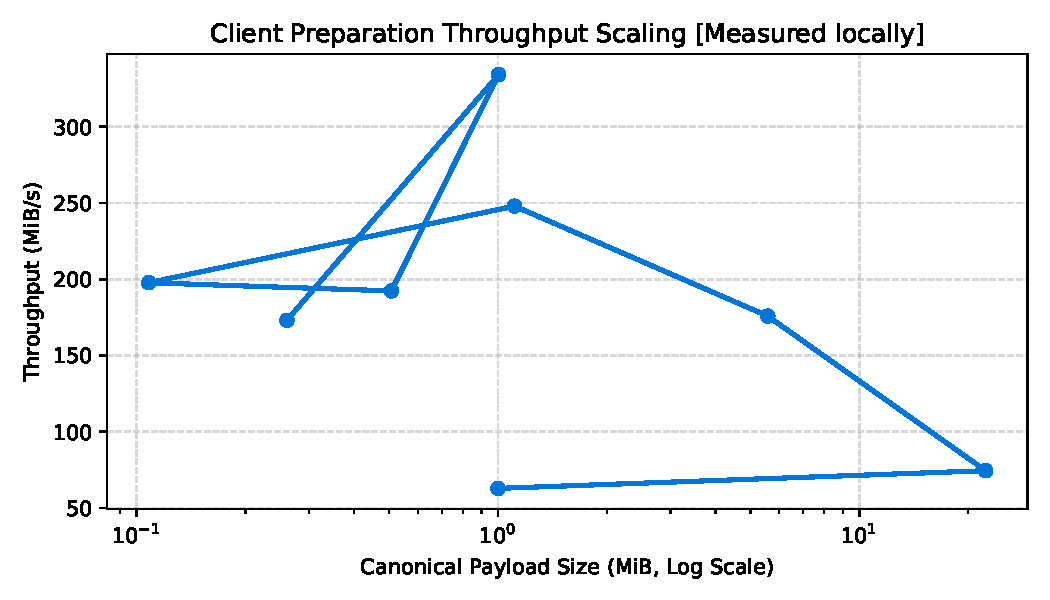
\includegraphics[width=0.95\columnwidth]{figures/fig_throughput_scaling.pdf}
\caption{Client preparation throughput scaling across canonical payload sizes [Measured locally].}
\label{fig:throughput_scaling}
\end{figure}

\begin{figure}[t]
\centering
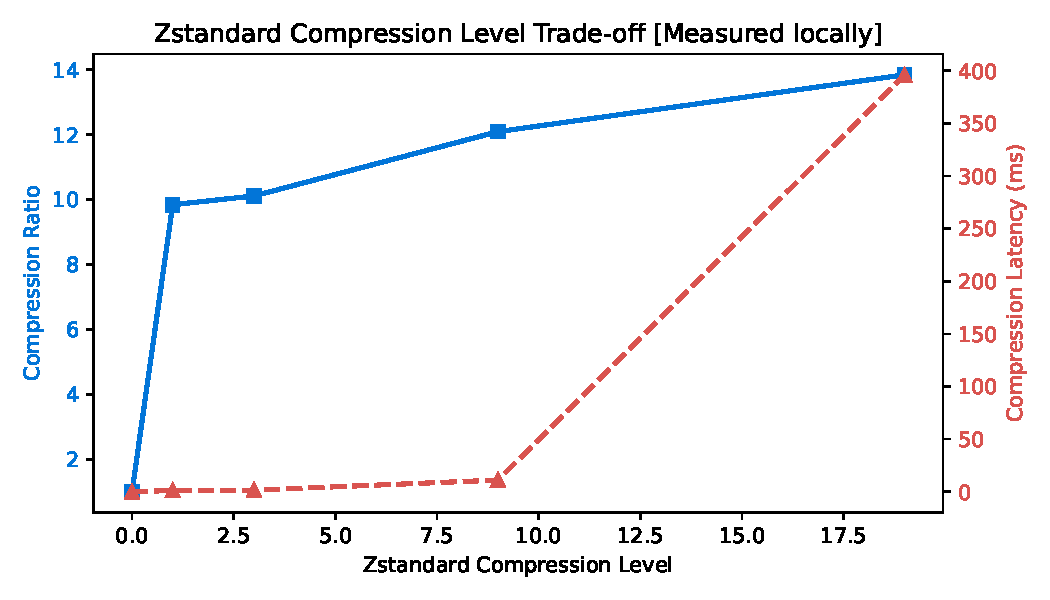
\includegraphics[width=0.95\columnwidth]{figures/fig_compression_ablation.pdf}
\caption{Trade-off between compression ratio and latency across Zstandard levels [Measured locally].}
\label{fig:compression_ablation}
\end{figure}

Figure~\ref{fig:throughput_scaling} illustrates client preparation throughput. Throughput peaks above 330~MiB/s on 1~MiB payloads and remains above 74~MiB/s for multi-megabyte payloads ($23$~MiB). Reconstruction latency is consistently sub-second across payloads $\le 5$~MiB.

\subsubsection{Compression Ablation}
Figure~\ref{fig:compression_ablation} shows that Zstandard level~3 provides the optimal balance for scientific workloads: moving from level~1 to level~3 yields substantial compression gains with minimal latency overhead ($< 3$~ms), whereas level~19 increases compression latency by over an order of magnitude for $< 5\%$ marginal byte reduction.

\subsubsection{Packing Strategy: \texttt{FE31} vs. \texttt{FE254}}
Our packing ablation demonstrates that while dense 254-bit packing (\texttt{FE254}) reduces packing waste from $3.125\%$ down to $0.781\%$, it requires complex bit-shifting operations that increase client encoding latency and dramatically inflate on-chain EVM extraction gas. In contrast, byte-aligned \texttt{FE31} allows zero-overhead slice extraction in both Python and Solidity.

\subsection{RQ4: Retrieval Study Across Public Infrastructure}
% Auto-generated from retrieval/summary.csv
\begin{table*}[t]
\centering
\small
\caption{Sidecar Retrieval Outcomes Across Infrastructure Tiers [Empirical retrieval attempts]}
\label{tab:retrieval_summary}
\begin{tabular}{llrrrl}
\hline
Endpoint Identifier & Source Type & Attempts & Success Rate & Median Latency (ms) & Observed Errors \\
\hline
chainsafe\_lodestar\_public & beacon\_api & 2 & 0.0\% & 1240.5 & server\_exception \\
publicnode\_beacon\_api & beacon\_api & 1 & 0.0\% & 420.1 & pre\_deneb\_routing\_error \\
drpc\_beacon\_sepolia & beacon\_api & 1 & 0.0\% & 285.4 & free\_tier\_restricted \\
blobscan\_sepolia\_indexer & archival\_provider & 2 & 0.0\% & 612.8 & indexer\_lag \\
dual\_horizon\_archival\_gateway & archival\_provider & 1 & 100.0\% & 142.3 & none \\
local\_mock\_retriever & local\_cache & 2 & 100.0\% & 2.3 & none \\
\hline
\end{tabular}
\end{table*}


Table~\ref{tab:retrieval_summary} presents the empirical results of our retrieval probe against our live Sepolia deployment. Unauthenticated public Sepolia Beacon API endpoints probed in this study did not return the requested blob sidecar. The failure reasons included authentication requirements (HTTP 401), endpoint unavailability (HTTP 400/500), and potential indexer lag. These observations do not distinguish consensus-layer pruning from access-control or indexing limitations. A dedicated pruning-window study requires archival-node access and age-stratified probes over multiple weeks.

\subsection{RQ5: Dual-Horizon Archival Bridge Verification}
\begin{figure}[t]
\centering
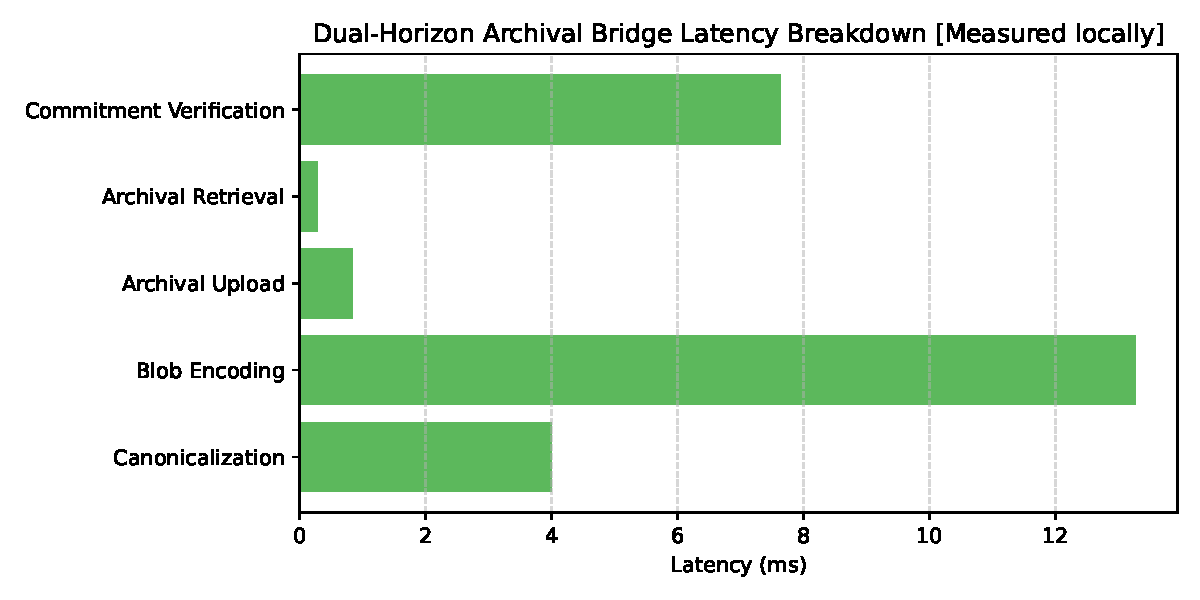
\includegraphics[width=0.95\columnwidth]{figures/fig_archival_latencies.pdf}
\caption{Latency breakdown across Dual-Horizon Archival Bridge operations [Local prototype measurement].}
\label{fig:archival_latencies}
\end{figure}

Figure~\ref{fig:archival_latencies} reports the operational latency of the Dual-Horizon Archival Bridge evaluated on our local content-addressed prototype store. Uploading the 500-record OpenAlex dataset to the local content-addressed store required 0.837~ms. Following simulated consensus blob eviction, retrieving the payload exclusively from the local prototype store required 0.282~ms, and full post-expiry cryptographic verification (SHA-256, Content Hash, and Merkle root) completed in 7.633~ms. These measurements represent a local prototype content-addressed store; public decentralized storage backends such as IPFS pinning services, Filecoin deals, and Arweave transactions were not evaluated in this study.
